\documentclass{article}

\usepackage{graphicx}
\usepackage{tikz}
\usepackage{tikzsymbols}
\usetikzlibrary{calc,patterns,shapes.geometric}
\pagestyle{empty}
\usepackage[margin=0pt]{geometry}
\geometry{papersize={14in,12in}}

\def\centerarc[#1](#2)(#3:#4:#5){\draw[#1] ($(#2)+({#5*cos(#3)},{#5*sin(#3)})$) arc (#3:#4:#5);}

\begin{document}
	\begin{figure}
		\centering
		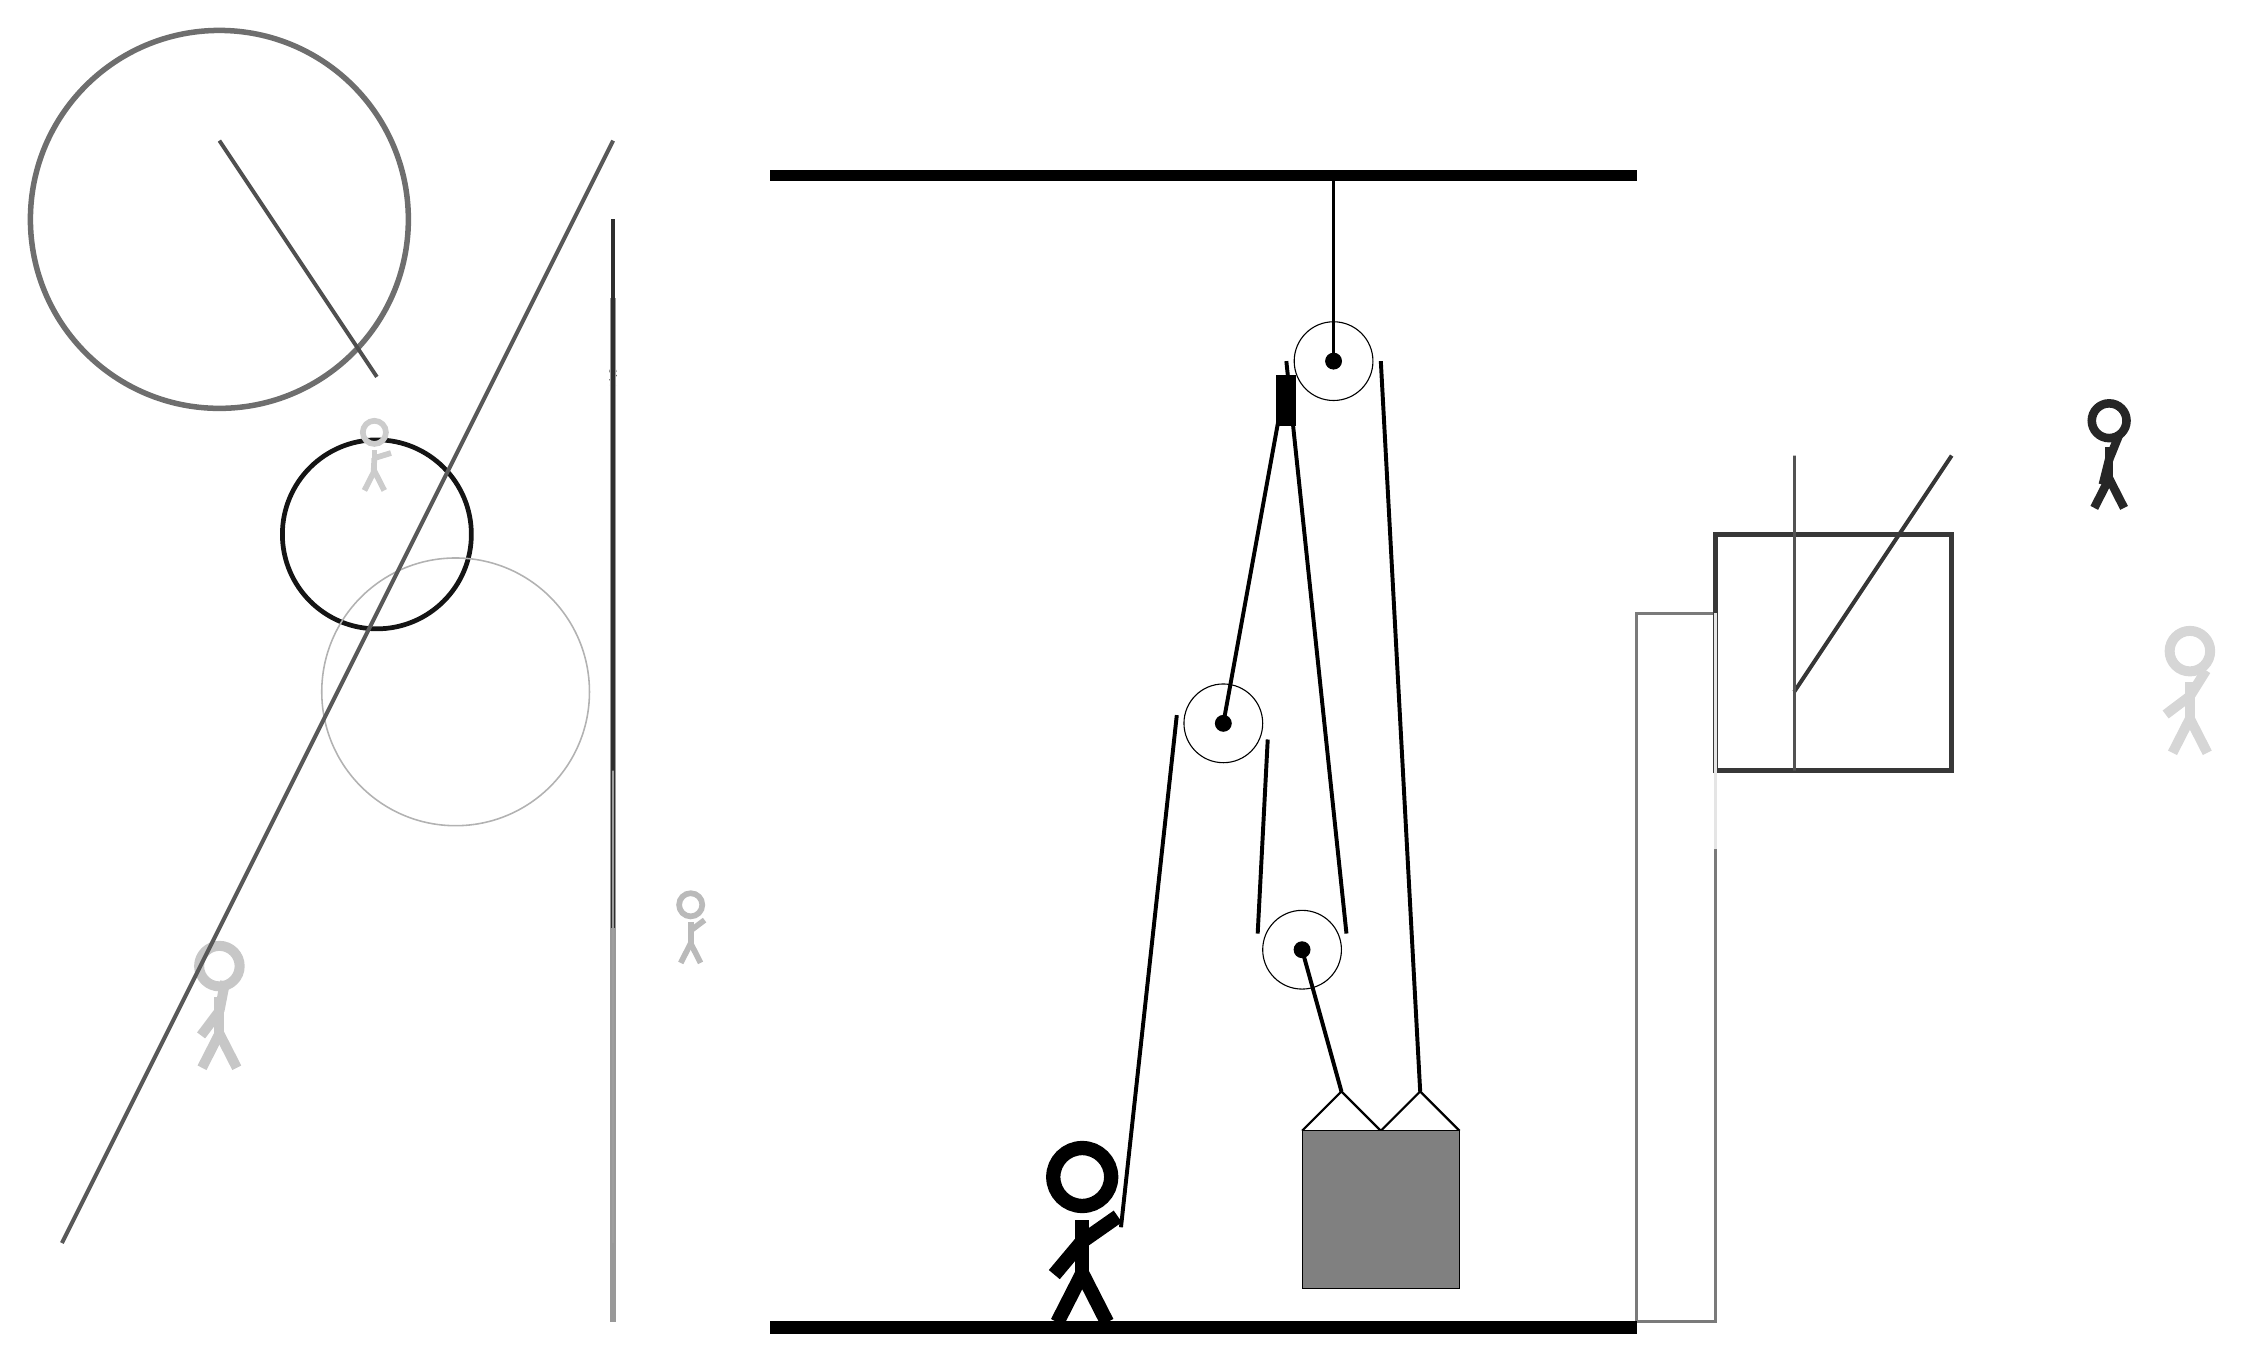
\begin{tikzpicture}
			%%%%% START %%%%%
			
			\draw[fill=black] (-6, 11.5) rectangle (5, 11.625);
			
			\draw (-0.25, 4.6) circle (0.5);
			\draw[fill=black] (-0.25, 4.6) circle (0.1);
			
			\draw (0.75, 1.725) circle (0.5);
			\draw[fill=black] (0.75, 1.725) circle (0.1);
			
			\draw (1.15, 9.2) circle (0.5);
			\draw[fill=black] (1.15, 9.2) circle (0.1);
			\draw[very thick] (1.15, 9.2) -- (1.15, 11.5);
			
			\draw[thick]  (0.75, -0.575) -- (1.25, -0.075) -- (1.75, -0.575) -- (2.25, -0.075) -- (2.75, -0.575);
			\draw[fill=black!50] (0.75, -0.575) rectangle (2.75, -2.575);
			
			\draw[line width=0.5mm] (-0.25, 4.6) -- (0.55, 9.0);
			\draw[line width=0.5mm, fill=black](0.45, 8.4) rectangle (0.65, 9.0);
			\draw[line width=0.5mm] (-1.55, -1.8) -- (-0.8409, 4.7042);
			\centerarc[line width=0.5mm](-0.25, 4.6)(-20:170:0.6);
			\draw[line width=0.5mm] (0.3138, 4.3948) -- (0.1862, 1.9302);
			\centerarc[line width=0.5mm](0.75, 1.725)(160:380:0.6);
			\draw[line width=0.5mm] (1.3138, 1.9302) -- (0.55, 9.2);
			\draw[line width=0.5mm](0.75, 1.725) -- (1.25, -0.075);
			\centerarc[line width=0.5mm](1.15, 9.2)(0:180:0.6);
			\draw[line width=0.5mm] (1.75, 9.2) -- (2.25, -0.075);
			
			\node at (-2, -1.9) {\Strichmaxerl[10][50][35]};
			
			\draw [line width=0.6mm, color=black!92](-11, 7) circle (1.2);
			
			\node[line width=0.6mm, color=black!66] at (-8, 9) {\Strichmaxerl[1][40][31]};
			\draw[line width=0.7mm, color=black!40] (-8, 10) rectangle (-8, -3);
			\draw[line width=0.5mm, color=black!82](-8, 2) -- (-8, 11);
			\draw[line width=0.5mm, color=black!79](7, 5) -- (9, 8);
			\node[line width=0.5mm, color=black!27] at (-7, 2) {\Strichmaxerl[4][90][37]};
			\node[line width=0.4mm, color=black!16] at (12, 5) {\Strichmaxerl[7][37][58]};
			
			\draw [line width=0.7mm, color=black!57](-13, 11) circle (2.4);
			\draw [line width=0.4mm, color=black!32](9, 2) circle (0.0);
			
			\node[line width=0.4mm, color=black!85] at (11, 8) {\Strichmaxerl[6][76][68]};
			\draw [line width=0.2mm, color=black!30](-10, 5) circle (1.7);
			
			\node[line width=0.2mm, color=black!22] at (-13, 1) {\Strichmaxerl[7][53][79]};
			\draw[line width=0.5mm, color=black!69](-11, 9) -- (-13, 12);
			
			\node[line width=0.6mm, color=black!20] at (-11, 8) {\Strichmaxerl[4][87][17]};
			\draw[line width=0.4mm, color=black!52] (5, 6) rectangle (6, -3);
			\draw[line width=0.6mm, color=black!78] (6, 4) rectangle (9, 7);
			\draw[line width=0.3mm, color=black!38] (-8, 4) rectangle (-8, -2);
			
			\draw[line width=0.4mm, color=black!68] (7, 4) rectangle (7, 8);
			\draw[line width=0.5mm, color=black!65](-8, 12) -- (-15, -2);
			\draw[line width=0.5mm, color=black!10](6, 3) -- (6, 6);
			
			\draw[fill=black] (-6, -3) rectangle (5, -3.15);
			
			%%%%% END %%%%%
		\end{tikzpicture}
	\end{figure}	
\end{document}